%-----------------------------------------------------------------------------------------------------
%TABLE OF CONTENTS (COMMENT OUT THIS SECTION IF YOU DON'T WANT TO ADD TABLE OF CONTENTS)
%-----------------------------------------------------------------------------------------------------
\tableofcontents 
\newpage
%-----------------------------------------------------------------------------------------------------

%-----------------------------------------------------------------------------------------------------
%REPORT TEXT
%-----------------------------------------------------------------------------------------------------
\chapter{Introduction}
  \chapter{Generation and selection of my own signals} 
  \section{Generation of signals}
  \subsection{Recording of signals}
  \begin{enumerate}
      \item  \textbf{Waveform of my voice signal --- my name  :}
      The utterance of my name 'abcd' is recorded using ................ (Please fill in all the details about the recording, properties of the recorded signal and further conversion to .wav format. List out the properties of the .wav file. Include as many details as possible). A segment of the voice signal from xx ms to yy ms is plotted in Fig. \ref{fig1}. the total number of samples corresponding to this is nnnn. 
      
    \begin{figure} [h]
    \centering 
    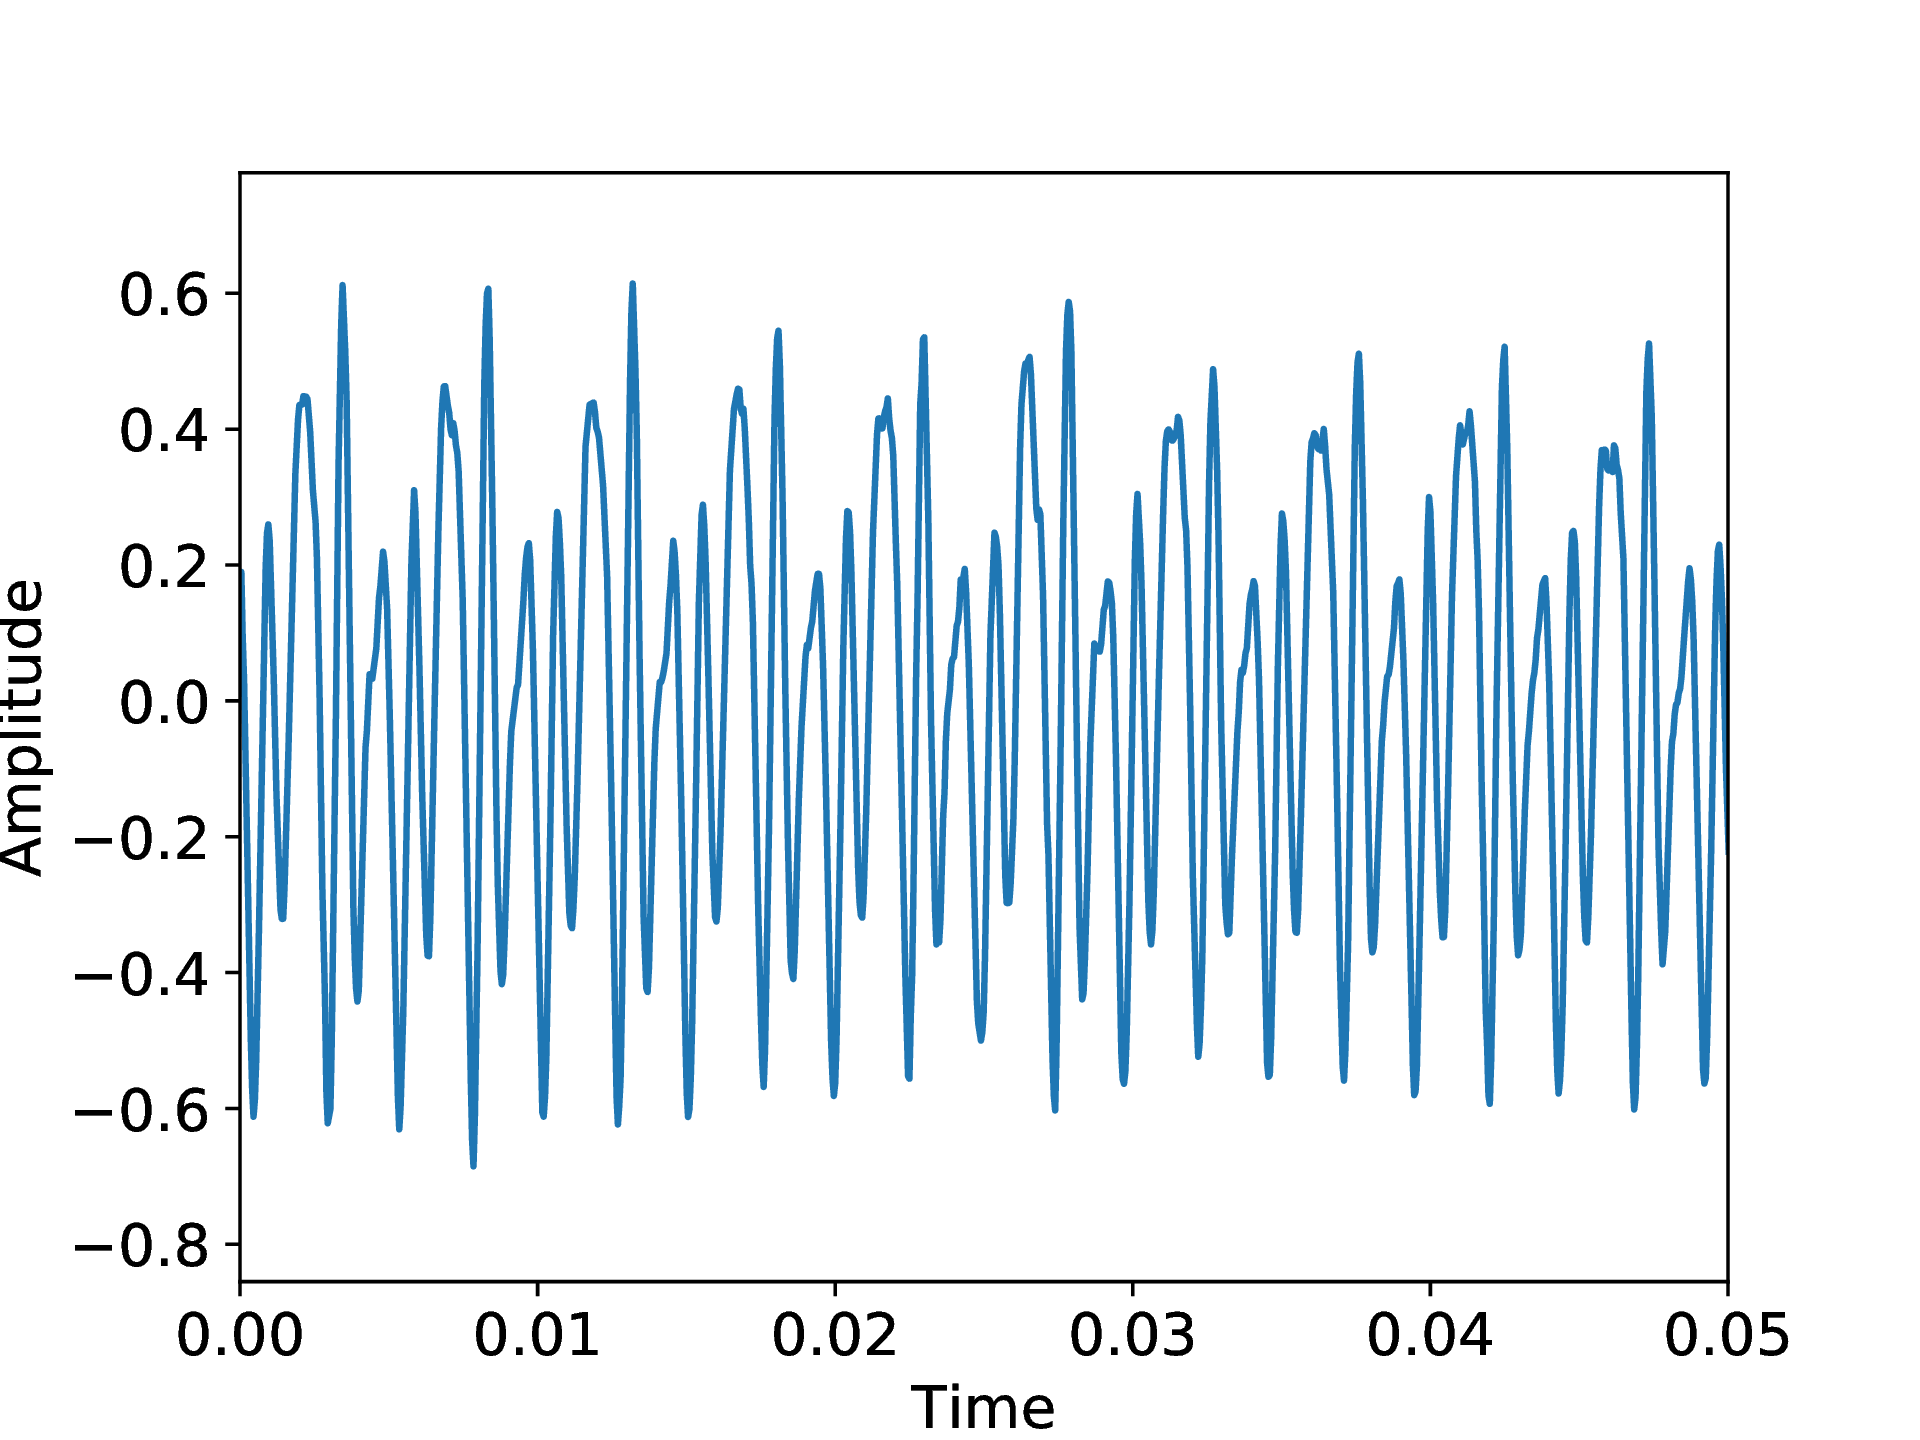
\includegraphics[width=0.55\textwidth]{edit/healthy_signal_plot.png}
 \caption{Plot of a segment of my voice sample corresponding to the utterance of my name --- yy ms}
 \label{fig1} 
 \end{figure}
 

      \item  \textbf{Waveform of my voice signal --- my roll number (R) :}
  
  The utterance of my roll number 'NN' is recorded using ................ (Please fill in all the details about the recording, properties of the recorded signal and further conversion to .wav format. List out the properties of the .wav file. Include as many details as possible). A segment of the voice signal from xx ms to yy ms is plotted in Fig. \ref{fig2}. the total number of samples corresponding to this is nnnn.
      
       \begin{figure}[h]
    \centering
    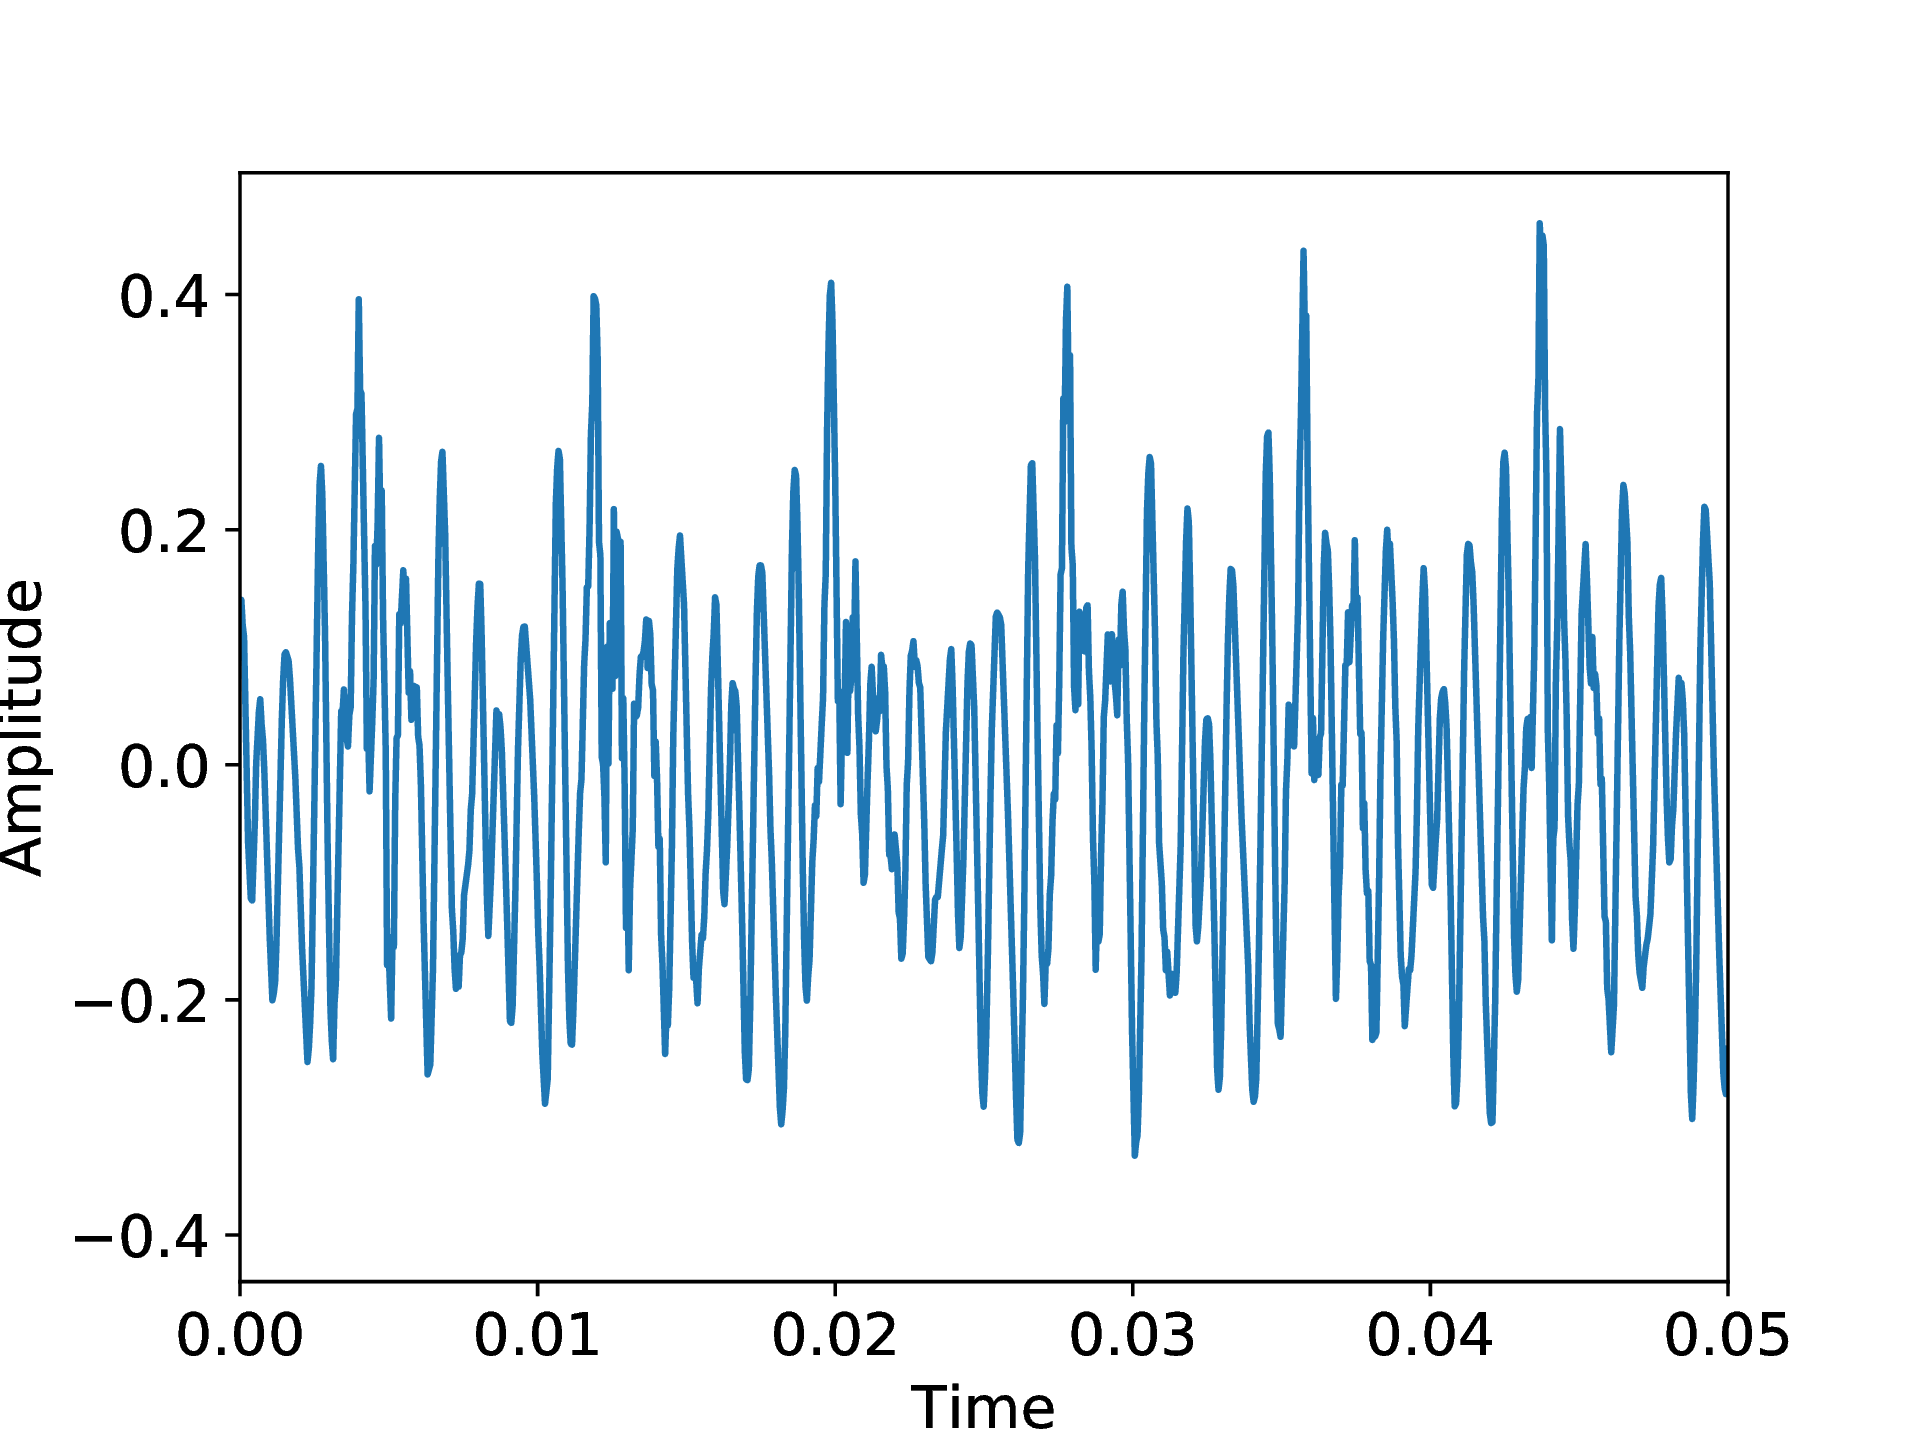
\includegraphics[width=0.55\textwidth]{edit/leukoplakia_signal_plot.png}
 \caption{Plot of segment of my voice sample corresponding to the utterance of my roll number}
 \label{fig2} 
 \end{figure}
      
      
      
      \item \textbf{Waveform of my voice signal --- a digit (A1)}
      \item \textbf{Waveform of my voice signal --- a digit (A2)} 
      \item  \textbf{Waveform of my voice signal --- a digit (A3)} 
      \item  \textbf{Waveform of my voice signal --- a sentence}
       \item \textbf{Waveform of my voice signal --- a music segment}
  \end{enumerate}
 
  \subsection{Synthesis of signals}
  
  \begin{multline*}
       x[n] = A_1*sin(2*pi*(R/f_s)*n) + A_2*sin(2*pi*(2*R/f_s)*n) +  \\ A_3*sin(2*pi*(4*R/f_s)*n)
  \end{multline*}
     
 
  \section{Selection of signals}
  
  \begin{enumerate}
      \item \textbf{Waveform of a music segment  -- 1}
      \item \textbf{Waveform of a music segment  -- 2}
      \item \textbf{Waveform of a music segment  -- 3}
  \end{enumerate}
 \section{Discussion and inference}
 
 Please analyse the plots and mention what all things you have observed 
  \chapter{Ex.2}
  \chapter{Ex.3}
  \chapter{Ex.4}
  \chapter{Ex.5}
  \chapter{Ex.6}
\chapter{Conclusion}
  
%-----------------------------------------------------------------------------------------------------

%-----------------------------------------------------------------------------------------------------
%BIBLIOGRAPHY (COMMENT OUT THIS SECTION IF YOU DON'T WANT TO ADD BIBLIOGRAPHY)
%-----------------------------------------------------------------------------------------------------
\begin{thebibliography}{}

\bibitem{reference_label1}
{2.Author}. \textit{1. Name of the document}. {Magazine/Journal/Publisher}.\\
\texttt{link to the web resource}

\bibitem{reference_label2}
{2.Author}. \textit{2. Name of the document}. {Magazine/Journal/Publisher}.\\
\texttt{link to the web resource}

\end{thebibliography}
%-----------------------------------------------------------------------------------------------------